% template.tex, dated April 5 2013
% This is a template file for Annual Reviews 1 column Journals
%
% Compilation using ar-1col.cls' - version 1.0, Aptara Inc.
% (c) 2013 AR
%
% Steps to compile: latex latex latex
%
% For tracking purposes => this is v1.0 - Apr. 2013

\documentclass{style/ar-1col}
\usepackage[utf8]{inputenc}
\usepackage{url}
\usepackage[numbers]{natbib}
\usepackage[inline]{enumitem}
\usepackage{multirow}
\bibliographystyle{plainnat}
\usepackage{todonotes}
\usepackage{caption}
\usepackage{comment}

\listfiles

\setcounter{secnumdepth}{4}

% Metadata Information
\jname{Xxxx. Xxx. Xxx. Xxx.}
\jvol{AA}
\jyear{YYYY}
\doi{10.1146/((please add article doi))}


% Document starts
\begin{document}

\newcommand{\shorttitle}{Precision pangenomics}
\newcommand{\firstauthorlastname}{Garrison}

% Page header
\markboth{\firstauthorlastname\ et al.}{\shorttitle}

% Title
\title{\shorttitle}


%Authors, affiliations address.
\author{%
  Erik \firstauthorlastname$^{*,\Delta,1}$,
  Jordan Eizenga$^{*,\Delta,1}$
  Simon Heumos$^2$,
  Jonas Sibbesen$^1$,
  Jana Ebler$^{5,6,7}$
  Glenn Hickey$^1$,
  Adam Novak$^1$,
  Xian Chang$^1$,
  Jean Monlong$^1$,
  Robin Rounthwaite$^1$,
  Shilpa Garg$^{8,9,10}$,
  Josiah D Seaman$^{3,4}$,
  Mikko Rautiainen$^{5,6,7}$,
  Tobias Marschall$^{5,6,7}$
  Benedict Paten$^1$,
  and Jouni Sir\'{e}n$^1$
%\affil{$^1$Genomics Institute, University of California Santa Cruz, Santa Cruz, CA, USA, 95064;
\affil{$^1$Genomics Institute, University of California Santa Cruz, Santa Cruz, CA, USA, 95064}
\affil{$^2$Quantitative Biology Center, University of Tübingen, Tübingen, Germany, 72076}
\affil{$^3$Royal Botanic Gardens Kew, Richmond, UK, TW9 3AB}
\affil{$^4$Queen Mary University of London, London, UK, E1 4NS}
\affil{$^5$Center for Bioinformatics, Saarland University, Saarbr\"{u}cken, Germany, 66123}
\affil{$^6$Max Planck Institute for Informatics, Saarbr\"{u}cken, Germany, 66123}
\affil{$^7$Saarbr\"{u}cken Graduate School for Computer Science, Saarbr\"{u}cken, Germany, 66123}
\affil{$^8$Department of Genetics, Harvard Medical School, Boston, MA 02215}
\affil{$^9$Department of Data Sciences, Dana-Farber Cancer Institute, Boston, MA 02215}
\affil{$^{10}$Department of Biomedical Informatics, Harvard Medical School, Boston, MA 02215}
\affil{$^*$email: erik.garrison@ucsc.edu, jordan.eizenga@ucsc.edu}
\affil{$^\Delta$equal contributors}
}

%Abstract
\begin{abstract}
Abstract text, approximately 150 words. 
\end{abstract}

%Keywords, etc.
\begin{keywords}
genome graph, variation graph, graph, pangenome, reference
\end{keywords}
\maketitle

%Table of Contents
\tableofcontents

\section{Introduction}

A \emph{pangenome} models the full set of genomic elements in a given species or clade \cite{sigaux2000cancer}.
This concept has been essential to microbiology, where genomic plasticity and diversity have made a pangenomic perspective indispensable \cite{tettelin2005genome,medini2005microbial}.
Usually, these analyses focus on the presence or absence of genes from given strains and the determination of a core (commonly present) and accessory (frequently absent) pangenome \cite{page2015roary}.

Pangenomic techniques have been applied outside of microbiology, such as in species contexts where genomes are small and often homozygous \cite{cao2011whole}, or in the publication or analysis of collections of novel sequences from a single species \cite{gao2019tomato,brohammer2018maize}.
However, most ``high-throughput'' analyses of large genomes depend on comparison of individuals to a common reference genome.

In recent years, reduced sequencing and \emph{de novo} assembly costs have supported the discovery of significant levels of large-scale genomic variation in many eukaryotic species, including humans \cite{li2010building,sudmant2010,sudmant2015integrated,chaisson2018multi}, arabidopsis \cite{alonso2016arabidopsis}, brewer's yeast \cite{yue2017contrasting}, and the fruit fly \cite{chakraborty2018hidden}.
These and other related findings encourage the application of pangenomic methods in any research setting where more than one individual is being analyzed \cite{computational2016computational}.

Here, we consider a new class of methods that approach the pangenome with precision, often at the resolution of single base pairs.
Unlike widely-applied pangenomic methods which consider genes as their fundamental unit, these precise pangenomic methods support the interrogation of collections of genomes and their relationships at any level of resolution.
They envision pangenomic analyses based on the full complement of DNA in the individuals under analysis, and aim to support downstream inference over variants of all types and scales, including small variation such as SNPs and indels in the same context as large structural variants gene gain or loss.

Scaling such techniques to operate on eukaryotic pangenomes has required significant effort in the development of new data models and algorithms.
Solutions to this problem are varied, but they often rely on graphical data structures that represent compressed versions of genomes and embed the many-to-many relationships inherent in the pangenome.

Not all methods expose this data structure as a coherent reference system.
They may instead use it internally to improve performance of a standard bioinformatic operation.
Even pangenomic models based on graphs are not necessarily equivalent, and many feature limitations that prevent them from representing certain kinds of genomic variation.

Although, these limitations have appeared expedient or even necessary to scale precision pangenomics to eukaryotic genomes, new algorithms and approaches for the construction and interrogation of pangenome graphs demonstrate that generic models can be scalable.
These results imply the possibility of simplifying and even expediting many bioinformatic analyses through the use of pangenomic reference systems and algorithms.

\subsection{Resequencing scales genome inference}

Our understanding of biological systems depends on our ability to see the relationships between genomes.
In the early days of genomics, when the cost of sequencing was high, expensive algorithms would be applied to relate all sequences in a given experiment to all others, typically yielding multiple sequence alignments.
These analyses were thus effectively \emph{pangenomic}, in their unified representation of all the genomic information in the analysis.
Each sequence was related to all others, and optimization procedures applied to the entire collection were used to obtain the most-parsimonious set of relationships between them.
\todo{JME: we should make sure that we tie back to this section when we discuss constructing pangenome graphs from alignments}

Increasing data scales have made such approaches prohibitively costly.
The arrival of high-quality reference genomes and low-cost short read sequencing has encouraged the use of \emph{resequencing}, wherein reads from each sample are aligned to a single common reference genome.
State of the art implementations of this process scale to support the combined analysis of tens of thousands of genomes \cite{Poplin_2017}, but they can only do so by relating each genome to a single common reference sequence.

\subsection{Resequencing implies reference bias}

Although efficient and conceptually simple, resequencing has a significant limitation.
The relationships between genomes are only visible for those sequences that are already close enough to those in the reference genome to be alignable.
%Significant variation between a new genome and the reference genome may be rendered invisible, or apparently less frequent, by the reference bias inherent in alignment.
The extent that sequence information from a given sample cannot be aligned to the reference causes \emph{reference bias}.
This effect is certainly strongest for structural variation or sequences that are absent from the reference system \cite{sudmant2015integrated}, but it can be relevant even for SNPs, which causes problems in alleles specific expression (ASE) quantification \cite{stevenson2013sources} and in the analysis of ancient DNA \cite{zhou2017antcaller}.

Given that this bias shapes the very genomic inference methods that we use to establish models of the truth \cite{zook2014integrating}, it is pervasive and will be difficult to evaluate without paradigmatic change in our sequencing and analysis techniques.
Recent studies have applied graph-based sequence alignment methods to show that this bias affects even the detection of small variation \cite{eggertsson2017graphtyper,Garrison_2018}, and that these methods can be used to mitigate its effect on the study of ancient DNA \cite{martiniano2019removing} and RNA sequencing data \cite{Kim_2019}.

\subsection{Human pangenomics}

Estimates based on short read sequencing data have placed the human pangenome at between 1\% \cite{li2010building} and 10\% \cite{sherman2019assembly} larger than the the GRCh38 human reference assembly.
Others have demonstrated several Mbp of sequence are present in each new individual and not in the reference \cite{li2010building,Steinberg_2016,Audano_2019}.
Although these estimates vary based on the author's definition of what constitutes novel sequence or allelic variation, we should expect them to rise as we consider larger cohorts of humans.
We might also gain greater insight into the placement and significance of these novel sequences when they are discovered in whole genome teleomere-to-telomere assemblies constructed from long single-molecule sequencing data \cite{miga2019telomere,Langley_2019}.

%Efficiently relating new sequences to such rich data resources will require the application of new kinds of resequencing and new models for bioinformatic analysis that support the inference of sensitive all-to-all relationships between large collections of large genomes.
%The genomics community is today working to determine what kinds of data models will allow researchers to fully exploit pangenomic data from humans and other species.
%Much attention has been given to the type of data structure which

%In addition to allowing the use of pangenomes in genome inference, the decreasing cost of whole genome assembly suggests that a new problem will arise in comparing whole genomes to each other.
%This issue of whole genome alignment or comparison suggests an end to the dominance of resequencing based tools, and implies the need for greater focus on methods that can efficiently process and report on whole assemblies.

In precision medicine, we seek accurate inference of a given patient genome.
Improving our prior model for what sequences we expect to see will reduce the time and cost required to infer a patient genome.
This does not only help us when we are genotyping known variants.
If most of the sequence and variation in any given individual is also found in the reference pangenome which we use, then we are left with a smaller set of sequences that do not map to the reference to consider when we attempt to infer novel variation.

\subsection{Pangenomic models}

A \emph{pangenomic model} is a data structure that represents the genomic sequences of a population, a species, a clade, or even a metagenome \cite{computational2016computational}.
The model serves as a central coordinating entity to describe the collection of sequences and genomes in the pangenome.
It may be indexed to allow for fast access to attributes of interest, such as to enable the matching of new sequences into it, or the extraction of genomes that that it was built from.
Pangenomic models have many shapes.

These models can take linear forms.
A linear reference genome in FASTA format may be augmented with smaller variation represented in auxiliary VCF files to build a pangenomic model.
A similar pangenomic model is the multiple sequence alignment, which can be built for any syntenic region of a collection of genomes.
However, both approaches have difficulty when representing complex and structural variation, such as copy number changes or translocations, and they must be augmented with \textit{ad hoc} information to do so.

Graphical pangenome representations naturally handle all kinds of variation, both small and large.
These models embed the pangenome in a graph where nodes are labeled with DNA sequences and edges represent linkages between successive nodes that occur in some set of the genomes.
The most basic sequence graph is acyclic, directed, and does not allow edges that go between the forward and reverse complement of the graph.
However, these restrictions must be relaxed to represent inversions and compact representation of copy number variations.
A generic sequence graph thus allows us to encode genomes and any kind of variation that might occur between them.

An efficient and popular approach is to break the input genomes into sequences of a fixed length $k$, yielding $k$-mers that together imply a regular and efficient graphical structure known as a \emph{de Bruijn graph}\footnote{It is the authors' opinion that ``de Bruijn'' should be written with a lower-case ``d'' when not starting a sentence, which seems to be the prevailing but not universal othrography in the literature.} (dBG).
This graph may be annotated, or colored, with information of the presence or absence of particular sequences in different individuals or biosamples, forming a \emph{colored} dBG.
dBGs have the advantage of representing the graph structure implicitly.
A dBG contains an edge for each pair of $k$-mers where the last $k-1$ bp of the first $k$-mer matches the first $k-1$ bp of the second.
They greatly simplify the process of pangenome construction, which can be built from any kind of input data that, and typically require only the specification of a length $k$ and an abundance threshold required to retain a particular $k$-mer.
However, they are lossy models that cannot reproduce their input, within which all repeated sequences shorter than $k$ are likely to collapse.

%In contrast to $k$-mer based models, which represent links implicitly,
\emph{Genome graphs} explicitly extend collections of linear sequences of arbitrary length with links that describe possible connections between sequences \cite{Paten_2017}.
These graphs can be seen as a kind of language model, in which each genome or sequence in the pangenome is a valid expression in the graph's language.
However, they also admit many sequences which are highly unlikely combinations of actual genomes.
To provide further structure to genome graphs, \emph{variation graphs} embed the observed linear sequences of the pangenome in the graph as \emph{paths}, or walks through the sequences of the graph \cite{Garrison_2018}.
Variation graphs are thus fully lossless pangenomic models that represent both a collection of sequences and their mutual alignment.
They are capable of representing all other kinds of pangenomic models, and provide stable coordinate systems based on the genomic sequences embedded within them.
%The set of sequences embedded within these graphs may be compressed into data structures that  \cite{Siren_2019}.

%The disadvantage of variation graphs is that their implementation has been difficult due to their generality.

%Such a data structure may be compressed
%Such sequence data can be represented in \emph{linear reference models}, like FASTA sequences, with variation represented in external files, but these approaches lack coherent representation of the relationship between sequences.
%Supporting 
%\footnote{\url{http://fastg.sourceforge.net/}}
%\footnote{\url{https://github.com/GFA-spec/GFA-spec}}
%In contrast to \emph{linear reference models}, like FASTA sequences, which require external information such as data in the variant call format (VCF)
%Pangenomic models encode both variation and sequence in a single model.


\subsection{Interfacing with the pangenome}

Pangenomes can be stored as collections of sequences in FASTA format.
Variant calls in VCF format may be added to such a collection to describe small or structural variants found in the pangenome.
Collections of FASTA sequences and alignments between them also imply a pangenomic data structure, which can be viewed in the form of a ``dot plot'' in two dimensions.
This approach breaks down when considering large numbers of related sequences, and is not commonly used as a way to convey a pangenome.

To encode graphical pangenomes, the community frequently employs the GFA\footnote{\url{http://gfa-spec.github.io/GFA-spec/}} format for sequence graph exchange.
GFA was originally designed as an interchange format for assembly methods, but the equivalence between graphical pangenomes and the data structures used by assembly methods allowed it to be repurposed as a pangenomic interchange model.

GFA provides no mechanism to express read alignments.
The vg toolkit has developed the GAM format, which generalizes the data model of the SAM/BAM format to work on graphical reference systems, and this has been taken up by a number of other alignment tools.
However, it lacks a simple text-based equivalent.
The recently-proposed GAF\footnote{\url{https://github.com/lh3/gfatools/blob/master/doc/rGFA.md#the-graph-alignment-format-gaf}} format (which generalizes PAF\footnote{\url{https://github.com/lh3/miniasm/blob/master/PAF.md}} to work on graphs) could serve this purpose.
GAF is related to rGFA\footnote{\url{https://github.com/lh3/gfatools/blob/master/doc/rGFA.md}}, which is a proposed restricted specialization of GFA for reference graphs.

%\todo[inline]{EG: here we should talk about which tools exist, and which data formats they read and write, with a figure too?}

%Each class of pangenomic model can be used as a basis to drive biological analyses.
%Implementations of particular analytical processes may produce or consume different types of pangenomic models.
%Methods to do so \todo{To do what?} are not fully equivalent.
%\todo[inline]{JME: I think this section should probably be expanded or cut}
%To provide perspective on the scope of these approaches, we consider their


%\subsection{Past reviews}

%\cite{computational2016computational}.

\section{Building pangenomic models}

\subsection{Constructing graphs} 
% Robin


\subsection{Indexing genome graphs}

A \emph{text index} maps query strings to their occurrences in the indexed text.
The occurrences are typically reported as a list of starting positions, from which one can easily determine the substrings matching the query.

Indexing the sequences encoded in a graph is more involved.
The number of $k$~bp paths often grows exponentially in $k$, and the number of distinct $k$-mers encoded as path labels may also grow exponentially.
Indexing or even enumerating all $k$-mers in the graph may be infeasible for reasonable values of $k$, and if the starting position of the occurrence reported by the index is in a complex region of the graph, there may be an exponential number of $k$~bp paths to investigate.

In practice, indexes for genome graphs must make trade-offs not encountered in text indexes.
In order to limit the exponential growth, the index may only support relatively short query strings.
Some indexes support longer queries by doing extensive preprocessing.
In other indexes, queries mapping to complex graph regions can be slow.
Instead of indexing the entire graph, the index may only contain $k$-mers from a simplified graph, or from specific paths of the graph.
While finding the path matching the query may be expensive in some cases, indexes typically save space by only reporting the starting position of the match.

\subsubsection{Indexing sequences using a graph}

The FM-index \cite{Ferragina_2005} is a text index, based on the Burrows--Wheeler transform (BWT) \cite{Burrows_1994}, that is frequently used with DNA sequences.
A variant of the FM-index, the RLCSA \cite{Maekinen_2010}, run-length encodes the BWT, allowing it to store and index a collection of similar sequences space-efficiently.
\citeauthor{Huang_2010}\ \cite{Huang_2010} observed that if we know a good global alignment of the sequences, we can use that information to make the index both smaller and faster.
\citeauthor{Na_2016}\ \cite{Na_2016,Na_2018} developed this approach further in their FM-index of alignment.
While the articles do not mention it, both \citeauthor{Huang_2010}\ and \citeauthor{Na_2016}\ use the graph induced by the alignment as a space-efficient representation of the sequences.

\subsubsection{Acyclic graphs}

% TODO "VCF graph" is a placeholder
GenomeMapper \cite{Schneeberger_2009} was the first graph-based read aligner.
It builds a directed acyclic graph from a reference sequence and a set of variants (VCF graph).
To index the graph, GenomeMapper uses a simple hash-based $k$-mer index, with $k \le 13$ to limit memory usage.

GCSA \cite{Siren_2014} was the first attempt to use the BWT with graphs.
It takes either a prebuilt DAG or generates one from a multiple alignment of sequences.
GCSA then applies a number of graph transformations that preserve the path labels in the graph \todo{Should we describe this as the ``language'' of the graph?}, until the nodes can be unambiguously sorted by the labels of the paths starting from the node.
This process balances on the fine line \todo{What does this mean, though? Is it linear in some graphs and exponential in others? Is it linear in practice and exponential in theory?} between linear and exponential.
If the complexity of the graph is above a critical threshold, the transformed graph quickly becomes too large to handle.

BWBBLE \cite{Huang_2013} is a BWT-based representation for VCF graphs.
Simple substitutions are encoded in the sequence using IUPAC codes, and the sequence is indexed using a normal FM-index.
Because each base can be encoded using 8 different characters, the search branches after every base.
Most branches can be quickly eliminated, however.
Insertions and deletions produce separate sequences, with selected amount of context around the variant.
The length of this context is an effective upper bound for query length.

The vBWT \cite{Maciuca_2016} took another approach to using the BWT for indexing VCF graphs.
It encodes variants as \texttt{(ref|alt1|\dots)} in the sequence.
When the search encounters a variant, it must branch to handle each allele separately.
While both BWBBLE and vBWT trade faster index construction for slower queries, a combination of the ideas can be quite practical \cite{Buechler_2019}.

\subsubsection{General graphs}

Some text indexes are based on Lempel--Ziv parsing or context-free grammars.
These indexes first find partial matches between the query string and the indexed phrases and then combine the partial matches into full matches using two-dimensional range queries.
In the hypertext index \cite{Thachuk_2013}, each node is a separate phrase.
Queries mapping to a single node or crossing a single edge can be matched efficiently, while finding mappings to complex graph regions can be slow.

\citeauthor{Bowe_2012}\ \cite{Bowe_2012} used techniques similar to GCSA for representing de Bruijn graphs.
If the graph transformations used in GCSA construction are stopped after $i$ steps, the resulting graph is equivalent to an order-$2^{i}$ de~Bruijn graph.
This de~Bruijn graph can be used to approximate the original graph.
There are no false negatives, but matches longer than $2^{i}$ may be false positives.
By using this approach, GCSA2 \cite{Siren_2017} attempts to support fast queries in arbitrary graphs.

While stopping the construction early allows GCSA2 to handle more complex graphs than GCSA, most graphs must be simplified before they can be indexed.
Typical simplifications include removing high-degree nodes and complex regions from the graph and replacing them with the reference sequence.
If a collection of haplotypes is available, the removed regions can be replaced with new subgraphs that contain separate paths for each distinct local haplotype \cite{Siren_2019}.
This way, the index will contain all $k$-mers from the haplotypes, while usually missing $k$-mers from their recombinations.

\subsubsection{Indexing graphs using sequences}

Instead of attempting to index the entire graph, it is often sufficient to index only selected paths in it.
CHOP \cite{Mokveld_2018} takes the paths corresponding to haplotypes and breaks them into smaller pieces.
The distinct pieces form an artificial linear reference, which can be used with any read aligner.
The process guarantees that any substring of the haplotypes of length $k$ is also a substring of one of the pieces.
As with BWBBLE, $k$ represents an effective upper bound for query length.

The Pan-genome Seed Index (PSI) \cite{Ghaffaari_2019} follows a similar approach with artificial paths.
Instead of using haplotypes, PSI uses a greedy algorithm to find a set of paths that covers as many $k$~bp windows in the graph as possible.
An index using these paths alone already works well in practice.

When a fully sensitive index is needed, PSI can reverse the role of the query strings and the graph.
While complex graph regions may contain an excessive number of $k$-mers, the reads mapping to them only contain a limited number of $k$-mers.
By indexing a batch of reads and searching for the complex regions in that index, all mappings of the query strings to the graph can be found with reasonable resources.


\subsection{Other population-ish succinct data structures}
% Erik

\subsubsection{de Bruijn}

% BOSS: \cite{Bowe_2012} (\cite{Roedland_2013} is similar)

\subsubsection{VCFs / genotype calls / haplotypes / binary matrices}

\subsubsection{gPBWT, GBWT}

% Jouni: I can write this


\subsubsection{Alignments / collections of strings}

% Jouni: We probably don't have space for this.




\section{Relating new information to the pangenome}

\subsection{Visualization}
% Adam
% Simon
% Josiah

\todo[inline]{SH: Abyss: Does not take GFA as input and only output from Abyss. 
Did not work on my machine.
I vote to leave this out.}\cite{nielsen2009abyss}
\todo[inline]{SH: NGS Graph Generator: This tool does only produce a graph as output from linear NGS data. I vote to leave this out of here, too.}\cite{nazarie_visualization_nodate_2019}

Visualization of pangenome graphs presents novel challenges, because their data structure is \begin{enumerate*}[label=(\alph*)]
\item convoluted,
\item multidimensional and
\item nonlinear.
\end{enumerate*} Traditional genome browsers exploit the one dimensional nature of linear sequence data and use the second dimension to paint annotations on the y-axis. This neatly organizes the data into a 2D rectangular shape. Graph genomes follow network visualizations which require three dimensions to render without overlapping lines.
Annotation tracks add still another dimension, forcing all graph visualizations to involve some degree of flattening.  
For data, graph visualization tools tend to target either genome assembly graphs or pangenome graph use cases.
An overview of such tools is given in Table \ref{table:1}.

\begin{table}[h!]
\centering
\caption{Table to test captions and labels}
\begin{tabular}{|c|c|c|c|c|} 
 \hline
 Tool & Layout Paradigm & Target Use Case & Scale of Data & Technical Notes \\ [0.5ex] 
 \hline
 \texttt{Bandage} & Force Directed & Genome Assembly & Gigabase Genome & Desktop \\ 
 2 & 7 & 78 & 5415 \\
 3 & 545 & 778 & 7507 \\
 4 & 545 & 18744 & 7560 \\
 5 & 88 & 788 & 6344 \\ [1ex] 
 \hline
\end{tabular}
\label{table:1}
\end{table}
\todo[inline]{SH: Start with our taxonomic system here. Then point to our fancy table.}

Bandage \citep{Wick_2015} is one of the most popular visualizations \citep{Mikheenko_2019}.
Originally designed for working with bacterial assembly and meta-assembly graphs \citep{Wick_2015}, it supports a wide range of formats and graph  paradigms.
It can be effectively used for interactively visualizing and exploring subregions of human-scale pangenome graphs \citep{Garrison_2019}, but its shortcomings become apparent at larger scales or with higher degrees of connectivity between graph regions \citep{Mikheenko_2019}.
The tool does have support for restricting the portion of the graph displayed to a particular ``scope'', but the tool is fundamentally built around laying out the graph under study in two dimensions, with all nodes represented, and panning and zooming around it.
Moreover, while the tool includes the ability to search for sequences in the graph, it does not have any ability to structure graph display using known linearization information.
\todo[inline]{JME: i'm worried some of these implementation details might be too in-the-weeds.
they have important implications, but i think this discussion would be more accessible to a general audience if we refocus it on the effects that these implementation decisions have on the user. SH: I agree here. Josiah and I will try to merge the Bandage and GfaViz paragraphs by "putting a lot of text in our table".}
\todo[inline]{JDS: Mention force directed graphs.  Mention Figure~\ref{fig:visualization}}

GfaViz is another desktop application for visualizing genome graphs which claims full support for newer GFA2 features, such as the gaps which allow GFA2 to represent scaffold graphs in addition to assembly graphs; these features are not available in Bandage, which supports only GFA1 \citep{Gonnella_2018}.
However, unlike Bandage, the GfaViz project has not released any binary builds or user interface screenshots of their application, so Bandage remains the more accessible tool.
\todo{JME: we should probably introduce the GFA format before mentioning it.  i wonder where we should do that...}

Departing from the desktop application model, two recent graph visualization tools, \texttt{SGTK} and \texttt{AGB}, are web applications in which the visualization is precomputed, lowering end-user system requirements \citep{Kunyavskaya_2018,Mikheenko_2019}.
SGTK is designed for visualizing scaffold graphs, which can have negative-overlap gaps between sequenced segments, and is based around the in-browser Cytoscape.js graph layout and rendering library \citep{Kunyavskaya_2018}.
It includes a potentially highly interpretable, reference sequence structured ``browser'' layout, but its use of Cytoscape.js appears to push it towards a generic circular node representation, rather than the purpose built bands of Bandage \citep{Kunyavskaya_2018}.
Moreover, its authors do not demonstrate its usability on large graphs, with the largest graph evaluated having only 923 nodes and 60,679 edges \citep{Kunyavskaya_2018}.

AGB has a similar overall design to SGTK, but makes different implementation choices.
It is relatively tightly tied to the assembly graph use case, requiring each (sequence-bearing) edge to be classifiable as ``unique'' or ``repetitive'' based on assembler annotation or sequencing coverage \citep{Mikheenko_2019}.
AGB is built around the idea of splitting up an assembly graph and visualizing portions of it, and features many ways to do this, including linear reference based and minimum edge cut based approaches \citep{Mikheenko_2019}.
On the backend, the tool is built around potentially megabyte-scale JSON files\footnote{\url{https://github.com/almiheenko/almiheenko.github.io/blob/8f4b2f8c7c498f04fa32f53f69b4bc59888a14f0/AGB/Flye_Human/data/repeat_graph.json}}, with no apparent provision for region-specific download, but the tool is still demonstrated to be scalable enough to handle human and other eukaryotic assembly graphs \citep{Mikheenko_2019}.

To deal with comprehensive pangenome graphs with sequence data, one design approach is to keep the browser-based client but to put more intelligence into the server.
This is the avenue taken by the Sequence Tube Map, which renders regions of pangenome graphs using a visual language inspired by transit system maps \citep{Beyer_2019}.
This tool operates at a much more magnified zoom level than tools designed to work with assembly graphs, and is useful for visualizing base-scale variation and short read mapping locations in human-chromosome-scale graphs.
However, its imposition of a local linear ordering and its limited graph simplification tools make it difficult to use on larger regions.

There is a difference in scale when moving from an assembly or scaffold graph to a comprehensive pangenome graph for even a species with as little diversity as humans.
While tools like SGTK and AGB have been demonstrated on graphs with tens of thousands of entities, the 1000 Genomes Project dataset contains 88 million known human variants \citep{1000_2015}, which gives a density over the 3 billion base human genome of about 34 bases per variant, and a comprehensive pangenome graph with tens to hundreds of millions of elements---a much larger graph than those that SGTK and AGB have been shown to work with.
Moreover, to achieve their single-megabyte-scale visualization file sizes for hundred-megabase- to gigabase-scale assemblies, these tools necessarily elide sequence information.


MoMI-G is a multi-scale genome graph browser currently under development \cite{yokoyama_momi-g:_2019}. It employs SequenceTubemap at nucleotide scale and integrates it into a  framework along side a circos plot for chromosome scale connections .\todo[inline]{Ref for circos -- https://www.ncbi.nlm.nih.gov/pubmed/19541911} 
The integration of multiple visualizations brings their strengths to bear on different areas.   A feature table is provided for filtering Structural Variants.  Annotation are shown alongside the  SequenceTubemap.

\todo[inline]{vg view force directed layout}
Other approaches to visualizing comprehensive pangenome graphs rely on restricting the problem in order to improve efficiency.
For example, by sorting the sequence-bearing nodes of the graph into a one-dimensional layout, the \texttt{vg viz} tool renders graphs of arbitrary size and complexity in linear time \citep{Garrison_2019}. 
The tool is designed around a base-level visual representation of the graph, and optimized for comparing long embedded paths in the graph, on the basis of which nodes they do or do not visit. 
It can be difficult to understand high-level or nonlinear structures in such a linearized layout. 
\texttt{ODGI viz}\footnote{\url{https://github.com/vgteam/odgi}} uses a layout very similar to \texttt{vg viz} and addresses scalability by binning hundreds of adjacent nodes together, thus reducing the resolution and making it possible to render gigabase pangenomes in a single image.

Figure~\ref{fig:visualization} provides a visual overview of the visualization methods surveyed here.
It remains an open problem to interactively visualize a comprehensive human pangenome graph, potentially including interchromosomal connections, at a variety of zoom levels, with modestly provisioned end-user hardware.
\todo[inline]{SH: This last sentence I would move to the discussion?}

\begin{figure}[h]
    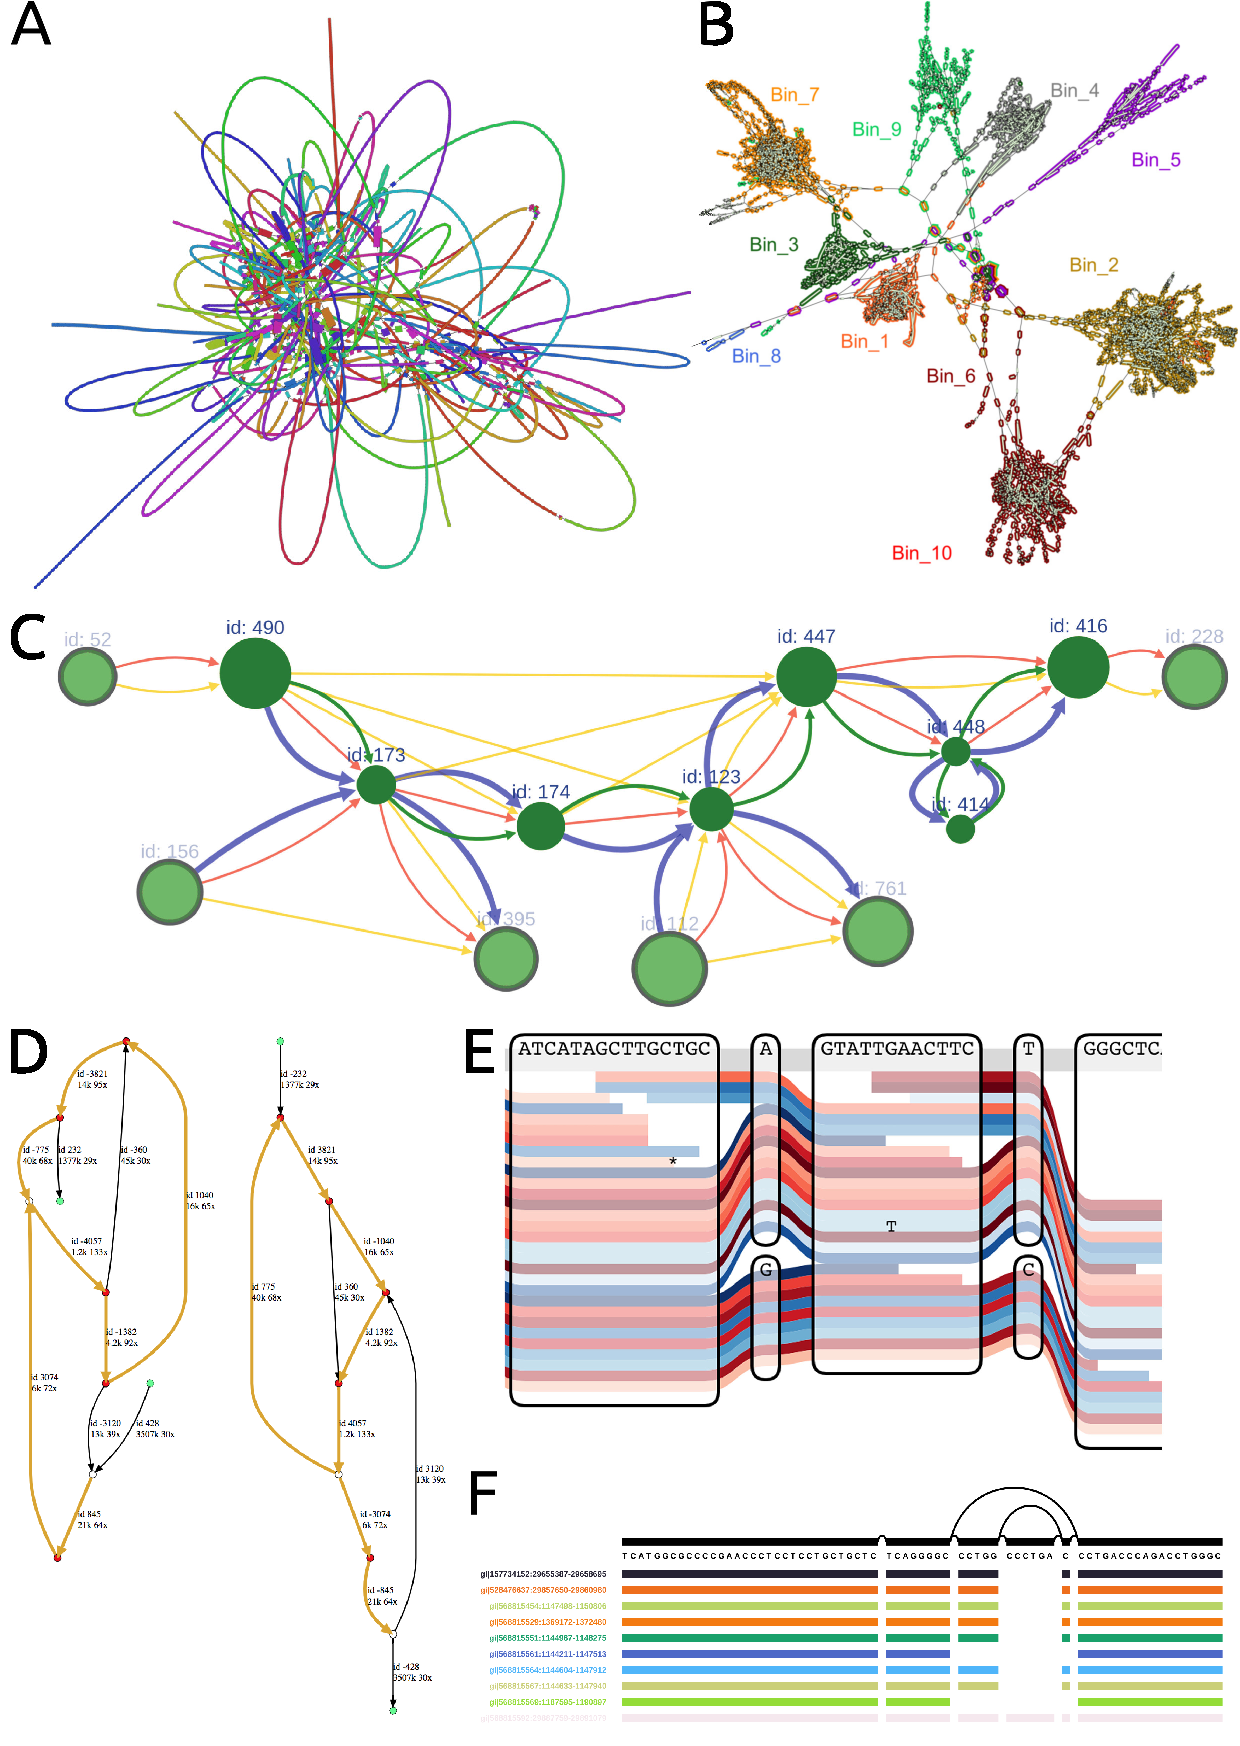
\includegraphics[width=0.9\textwidth]{figures/visualization.pdf}
    \caption{\label{fig:visualization} An overview of several approaches to visualizing assembly, scaffold, and comprehensive pangenome graphs.
\textbf{A:} Bandage, adapted from \cite{Wick_2015} supplementary section~6.
\textbf{B:} GfaViz, adapted from \cite{Gonnella_2018} supplementary figure~S4.
\textbf{C:} SGTK, adapted from \cite{Kunyavskaya_2018} figure~1.
\textbf{D:} AGB, adapted from \cite{Mikheenko_2019} supplementary figure~S3.
\textbf{E:} Sequence Tube Map, adapted from \cite{Beyer_2019} figure~2.
\textbf{F:} \texttt{vg viz}, adapted from \cite{Garrison_2019} figure~2.20.}
\end{figure}

% Go back and talk about ABySS-Explorer (2009) and its "polar" graphs and wiggly sequence edges?
% Bandage: cross-platform native application
    % Versatile and popular
    % Client-only
    % Could look up a reference but not view vs it
% GfaViz: C++/Qt tool with full GFA1/2 support
    % Has a GUI but no screenshots or binaries
    % Can show cool stuff like reads connected to their assembly contigs
% SGTK
    % build-view model
    % Cytoscape.js or genome browser linear-structured
    % designed for scaffold graphs (more processed?)
    % Not proven on large graphs; only shown going up to 100s of nodes
% AGB: auto-subgraphs (to 100 nodes) and simplifies assembly graphs
    % js GraphViz based
    % Still uses a build-web-page model
    % Kind of tied to assemblies (notion of repetitive vs non-repetitive edges)
    % Can view vs a reference
    % Scales to C elegans at least
        % O(300 * 100 = 30000) nodes
    % Appears to be structured around megabyte-scale GraphViz graphs https://github.com/almiheenko/almiheenko.github.io/tree/master/AGB
        % No LOD-ing on the backend for efficient download, but not a problem at the scale of 10s of thousands.
% Tube Map
    % Client-server model: requires a server, but can use server resources to crunch the graph
    % Designed to impose a left to right local ordering that orients the edges in a hopefully sensible way
    % Scales well to millions of nodes, demonstrated on partial human pangenome graph references


%\citep{Wick_2015} : Bandage
%\citep{Gonnella_2018} : GfaViz
%\citep{Kunyavskaya_2018} : SGTK
%\citep{Mikheenko_2019} : AGB
%\citep{Beyer_2019} : TubeMap
%\citep{Garrison_2019} : Thesis

\subsection{Finding structures in pangenome graphs}
% Jordan

\todo[inline]{JME: We need to decide whether to do this section}

\subsection{Graph alignment algorithms}

Often, genomic sequence data can only be interpreted in the context of other sequences. 
For this reason, sequence comparison is at the core of many genomic analyses, and sequence alignment is the essential method for doing so. 
However, classic alignment algorithms like Smith-Waterman \cite{Smith_1981} do not directly apply to sequence graphs. 
Accordingly, the increasing prominence of genome graph methods has been fueled by fundamental algorithmic research in graph alignment, and it has also spurred further research.
\todo{JME: this lead-in is redundant with the introduction, but it could be rewritten to tie into that content.
i'll do that later.}

The trend in the graph alignment research is toward greater generality and faster run time. 
The generality comes in two main forms. 
First, algorithms apply to increasingly general classes of graphs. 
The foundational genomic sequence graph alignment algorithm, partial order alignment, applied only to graphs without cycles \cite{Lee_2002, Grasso_2004}. 
\todo{EG: this is not accurate. Myers showed cyclic to cyclic graphs in 1990. This is also described in \emph{Biological sequence analysis}. \\ JME: i'm aware, but i want to tell the story of those algorithms being lost and rediscovered in the graph genome space. i can probably find a more }
More recent research has discovered algorithms that align to graphs with any shape \cite{Antipov_2015,Rautiainen_2017,Jain_2019a}. 
Second, graph alignment researchers have developed algorithms that use increasingly general scoring functions. 
Some earlier algorithms require restricted scoring functions to achieve efficiency \cite{Rautiainen_2017}, but recent contributions have used the less restricted scoring functions that are required to produce biologically meaningful alignments in many contexts \cite{Jain_2019a}.

Graph alignment research also has improved the algorithms' run time. 
The first algorithms required acyclic graphs in order to run at comparable speed to linear sequence alignment algorithms \cite{Lee_2002}. 
Later optimizations simply ran slower on general graphs \cite{Kavya_2019}
It has now been shown that graph alignment can run at the same speed as linear alignment (in the computer scientist's sense of ``Big-O'' asymptotics).
\todo{EG: Let's just use the actual notation here.}
This is believed to be essentially optimal \cite{Jain_2019a,Equi_2019}. 
In fact, these results were already known in other fields.
Many of the advances in this space came from rediscovering analogs to the graph alignment problem in the related areas of regular expressions and hypertext \cite{Myers_1989,Amir_1997}. 
In addition to these theoretical results, researchers have also developed modified algorithms that run quickly the practical context of real-world computer architectures \cite{Suzuki_2018,Rautiainen_2019,Jain_2019b}.

From a practical standpoint, the primary benefit of the research in alignment algorithms has been in aiding the design of mapping tools. 
Graph alignment algorithms are a central component of the graph mapping tools described below.

\subsection{Genome graph mapping}

Once a significant barrier to pangenomics research, the field now provides an array of well-performing, increasingly efficient read mapping tools for genome graphs. 
In some ways, the current landscape resembles the early days of short reads mappers for conventional references. 
A diversity of tools are now available, each experimenting with different algorithmic ideas. 
However, the field has not yet coalesced around any standard tool in the way conventional mapping now has around BWA-MEM \cite{Li_2013}. 

To the extent that a standard exists, it is currently VG \cite{Garrison_2018}---at least in the sense that later tools have largely chosen it as a point of comparison for their own performance \cite{Guo_2018,Kim_2019,Vaddadi_2019,Rautiainen_2019b}. 
It remains to be seen if VG will retain this position, or if another tool will emerge as the standard, or if a diversity of tools will be continue to be used. 
The ideal situation is probably the latter. 
The available tools represent a menu of tradeoffs that could be matched to different studies' unique requirements.

Invariably, genome graphs mappers make use of the seed-and-extend paradigm that has also been successful for linear references.
This methodology consists of first indexing the reference for exact match queries.
Then, the index is queried with a sequencing read for exact match ``seeds'', which are used to narrow in on small regions of the reference.
Expensive approximate-match alignment algorithms can then be targeted at these smaller regions to ``extend'' the seeds into full alignments. 
As this description suggests, a mapping tool's features are in large part determined by its choice of an indexing method and an alignment algorithm.
Genome graph indexing and alignment have both been active areas of research, as discussed above.
In addition, some tools employ an additional step to cluster seeds by their position on the graph before aligning.
While common for conventional mappers, the clustering step has proven challenging in genome graphs, and some tools omit it entirely.



%exhaustive traversals: debga-vara, 7 bridges

% general themes
%-need to control memory
%-need to employ approximate alignments
%-improved performance mapping to variants and calling variants from mappings
%-historically, divided into variation graph mapper

%IDEA: first commonalities, then differences



One major point of distinction between mapping tools is the type of graphs they were designed for. 
Several tools apply only to acyclic variation graphs, often the largely linear graphs that are formed by adding substitution and indel variants to a linear reference. Examples include GenomeMapper (an early forerunner) \cite{Schneeberger_2009}, Seven Bridge's Graph Genome Aligner \cite{Rakocevic_2019}, HISAT2 \cite{Kim_2019}, and V-MAP \cite{Vaddadi_2019}. 
Another set of tools focus on de Bruijn graphs: BGREAT \cite{Limasset_2016}, deBGA \cite{Liu_2016}, BrownieAligner \cite{Heydari_2018}, and GraphAligner \cite{Rautiainen_2019b}. 
Most of these were developed in parallel to recent pangenomics research, often with motivations in genome assembly. 
VG \cite{Garrison_2019} appears to be the only tool with open ambitions of mapping to both acyclic variation graphs and more complex genome graphs, although GraphAligner is valid on general graph topologies as well.

The majority of these tools emphasize mapping short-read \emph{next-generation sequencing (NGS)} data. 
Most likely, the motivation for doing so is the same as why NGS remains the standard for conventional resequencing experiments; the price point currently favors it. 
In this sense, pangenomic graph mappers essentially represent an incremental technical improvement over previous pipelines, albeit a very important one. 
To our knowledge, GraphAligner and V-MAP are the only graph mapping tools that explicitly targets high-error long read sequencing data\cite{Rautiainen_2019b, Vaddadi_2019}, although others are in development \cite{Li_2019}.

% a paragraph about the approximations used?

Among the graph mappers that emphasize variation graphs, a theme has emerged about their accuracy. 
They typically do not improve mapping accuracy over the entire genome compared to state-of-the-art linear mappers. 
However, they do significantly improve read mapping accuracy \emph{over variants} \cite{Garrison_2019, Rakocevic_2019, Kim_2019}. 
In this, we see a concrete example of pangenomic methods mitigating reference bias. 
The unimproved (and often slightly diminished) performance over the rest of the genome probably indicates a combination of the relative nascency of the graph mapping tools and the burden of more complicated computational heuristics.

The actual algorithms that each tool employs vary greatly. 
For indexing, most graph mapping tools have opted for some variation of a $k$-mer table. 
In the case of de Bruijn graph mappers, this is an especially attractive option since the $k$-mers also implicitly define the edges of the graph. 
This may be why all of the de Bruijn graph mappers listed above use this strategy \cite{Holley_2012, Limasset_2016, Liu_2016, Heydari_2018, Rautiainen_2019b}. 
Additionally, GenomeMapper, Seven Bridge's mapper, and V-MAP seed with $k$-mer tables \cite{Schneeberger_2009, Rakocevic_2019, Vaddadi_2019}. 
The remaining mappers use succinct text indexes.
VG uses the GCSA2 \cite{Siren_2017} and a longest-common-prefix array, which enable very specific maximal-exact-match queries.
The cost is that the index is large, which contributes to VG's high memory utilization \cite{Garrison_2019}.
HISAT2 uses a modified GCSA \cite{Siren_2014}  that also encodes the graph structure itself.
This helps give HISAT2 an impressively low memory footprint at the expense of a somewhat more limited set of queries \cite{Kim_2019}.

Most de Bruijn graph mappers have used searches through the graph to make alignments.
deBGA exhaustively enumerates paths, but reduces the space of sequences to align to with a clustering step.
Its core alignment algorithm is actually a sequence-to-sequence algorithm applied to each path \cite{Liu_2016}.
BGREAT addresses the combinatorial complexity of the extension step by greedily choosing a path in the graph.
This is fast, but provides no optimality guarantees, and their algorithm does not support indels \cite{Limasset_2016}.
Unfortunately, neither deBGA nor BGREAT compare their performance to any graph-based tools, and the somewhat unnatural context for the linear mappers they compare to makes their evaluations hard to interpret.
BrownieAligner also exhaustively explores paths out from a seed, but it uses a branch-and-bound algorithm to prune the search space along the way.
It also has a unique trick of choosing paths partially based on a Markov model trained on the reads.
This is essentially a limited form of read-backed phasing.
According to the authors' analysis, BrownieAligner is more accurate than deBGA and BGREAT, but BGREAT tends to be more memory efficient, and deBGA tends to be faster \cite{Heydari_2018}.
Finally, GraphAligner is the only de Bruijn graph mapper to take advantage of recent research into graph alignment algorithms.
It uses a banded alignment algorithm to achieve impressive speed aligning long reads to genome graphs \cite{Rautiainen_2019b}.

While few of the de Bruijn graph mappers employ graph-based alignment algorithms, most variation graph mappers do. One exception is GenomeMapper, which aligns to all paths out from a seed. However, GenomeMapper also seems to be unmaintained since 2009, and it has heuristics that are better suited to earlier NGS technologies \cite{Schneeberger_2009}. 
Seven Bridges' mapper, VG, and V-MAP all employ some version of partial order alignment \cite{Rakocevic_2019, Garrison_2019, Vaddadi_2019}. 
Seven Bridges also tries to find a near-match using a depth-first search algorithm before resorting to costly alignment algorithms \cite{Rakocevic_2019}. 
The HISAT2 alignment algorithm is a complex set of heuristics that lean heavily on the exact match seeds from its optimized index. 
This makes it exceptionally fast, although it also can hurt alignment quality around indels. 
In general, VG compares favorably to other tools in terms of accuracy on NGS data. However, most comparisons point out that it is quite demanding on computer memory and often slower than the alternatives \cite{Kim_2019, Vaddadi_2019}. 
V-MAP uses distance-based heuristics on acyclic graphs to efficiently cluster seeds. 
This allows it to align high-error long reads more efficiently than VG, although to our knowledge there has yet to be a published comparison to GraphAligner \cite{Vaddadi_2019}.

%\todo{JME: why are we going into so much detail about HISAT2 compared to the other tools?}
%HISAT2 is a BWT-based mapping algorithm that uses an adaptation of the Ferragina-Manzini (FM) index, a hierarchical graph FM index (HGFM).
%\todo{JME: it actually uses a GCSA, not a standard FM index}
%An FM index is a compressed representation of the graph that is optimized for substring searching.
%The HGFM is comprised of two FM indexes: a global index of the entire genome and local indexes of smaller portions of the genome and their variants.
%Repeat sequences are combined into a separate index, keeping only one copy of each repeat so sequences in repetitive regions are only aligned once.
%Alignment is done by searching the FM indexes, starting with the global index.
%
%
%Each of these graph alignment tools has demonstrated an increase in sensitivity over mapping to a standard linear reference.
%\todo{JME: what tools are you referring to with "each"? you've only referred to one tool}
%GenomeMapper, vg map, Seven Bridges' mapping algorithm, and HISAT2 are primarily short read mappers.
%\todo{JME: i think 7bg's tool is called Graph Genome Aligner}
%GraphAligner is a long read mapper and V-MAP is used for both.
%V-MAP doesn't align reads itself but finds a small subgraph that a read can be aligned to using existing mappers. 
%HISAT2 and vg can align both RNA and DNA.


%VMAP
%-only for DAGs
%-minimizer of most paths for index
%-linear embedding based on distance from source node for clustering
%-finds better mappings than vg for short reads, worse for long reads
%-significantly faster than map in their evaluations
%-uses GSSW for alignment

%GraphAligner
%-focus on long reads aligned to de bruijn graphs
%-does not chain seeds
%-indexes minimizers on only  node sequences, not paths
%-uses banded version of bit-parallel algorithm with tweaks
%-banding is based on x-drop rather than classic parallelogram shapes
%-hard caps on amount of dp and priority queue in tangled regions
%-actually suitable for arbitrary graphs, i think
%-very fast for what it does

%7bg
%-referred to as Genome Graph Pipeline and Graph Aligner
%-k mer hash table along all paths, but with cap on total number of edges, thinned
%-employs clustering, but sketchy on details
%-multi-stage alignment:
%	-first gapless alignment with graph-aware BITAP algorithm
%	-GSSW if there are novel indels
%-only supports VCF DAGs
%-better precision and recall compared to bwa on reads with variants

%genomemapper
%-presented as a technique for mapping to species with high polymorphism
%-discuss reference bias
%-hash based indexing - short k-mers (5 to 13)
%-memory mapped index
%-does not use vcf, seems to use IUPAC for snps
%-some effort toward making a bit-efficient encoding
%-3 stage alignment
%	-find exact matches with k-mers
%	-extend to nearly-identical matches
%	-banded alignment if this fails
%-I don't get how the alignment handles the branching of the graph...
%	-oh, it seems this seeding step only applies to blocks, then tree unrolling
%-for some reason does intra-read task parallelism for tree unrolling
%-demonstrate advantages for indel calling and alignment

%hisat2
%-VCF style graphs, insertions limited to 20 bp
%-GFM representation, based on Jouni's prefix-sorted graphs
%-hierarchical index
%	-one global index with reference and many variants
%	-thousands of 50kb local indexes, partially overlapping
%	-in hisat1 paper, local indexes are presented as a way to find smaller matches in local regions near splice sites
%-50-60% slower with 14M variants that itself without variants
%-obtains greater accuracy on reads containing variants
%-low memory usage: 6.2 GB (self-indexed)
%-compress repeat sequences in the genome and align to them with BWT-FM index
%	-identified by a k-mer count of 100-mers
%	-construct a de bruijn graph of frequent k-mers and then do greedy walks in it to identify sequences
%-i wonder if the reason they need to do this business with the repeats is that the strategy of finding a fixed number of exact matches and relying on pidgeonhole principle performs poorly against the repeat content of the non-coding genome
%	-do they actually do this method? the hisat supplement describes a pretty complicated set of heuristics

%debga-vara
%-emphasizes RAM usage
%-uses landau-vishkin algorithm (fast approximate algorithm with < k edits)
%	-banded, edit distance penalty
%-seem to emphasize low memory footprint
%-possibly doing tree unrolling? or maybe aligning to a suffix tree?
%	-sounds to me like tree unrolling with skips for indels
%-seems to only index the reference, not any variation
%-claims faster speed that BWA-MEM and better performance
%-the results they get on certain tools make me question the whole evaluation
%-i get the sense that when they say a problem is NP-hard, they actually mean that they wrote an exponential algorithm for it

%minigraph
%-does not yet give base-level alignment
%-intended for coarse graph without too much small variation
%-minimizer hash table for seeding
%-linear chains on nodes, followed by multi-path distance search between chains
%-

%make a section about controlling memory usage? -- emphasis of debga vara and hisat2

%gaffe?

%ggmap/bgreat - greedy matching from each overlap seed, align to entire unitigs at a time
%-start a new mapping for each "first seed"
%-find that blastgraph has serious scalability problems

%it seems all of the DBG methods use some kind of DFS type search (possibly greedy or BnB)

%liu-debga
%-index all kmers of unitigsg


%\subsection{De Bruijn graph mappers}
%% Adam
%
%% Style Note: apparently de Bruijn Graph should be lower case unless otherwise required to be capitalized.
%
%In addition to mappers designed to map to general graphs, a selection of mappers designed to map specifically to de Bruijn graphs, or to compacted de Bruijn graphs\todo{Did we define this already?}, have also been developed.
%
%One of the first of these, BlastGraph from 2012, uses an edit distance alignment metric for scoring, and finds all matches in the graph within that edit distance \citep{Holley_2012}.
%However, it seems better suited to search than to mapping to support resequencing; but it is only shown running on up to 10,000~reads at a time \citep{Holley_2012}.
%The actual alignment algorithm uses a hash-table-based seed index combined with a recursive-depth-first-search-based extension step, and is shown applied to de Bruijn graphs and ordinary sequence graphs \citep{Holley_2012}.
%\todo{Can we move this to the previous section since it doesn't really do anything de-Bruijn-specific?}
%
%\citeauthor{Holley_2012} do not discuss the algorithmics of their alignment approach, beyond demonstrating that it is sufficiently fast in practice \citep{Holley_2012}.
%In \cite{Limasset_2016}, \citeauthor{Limasset_2016} present a proof that the ``de Bruijn Graph Read Mapping Problem'' (when looking for acyclic mappings) is NP-complete, by a reduction of the Hamiltonian Path Problem, through a Traveling Salesman Problem variant, and then through a gapless, acyclic read-to-sequence-graph mapping problem \citep{Limasset_2016}.
%This realization of NP-completeness goes on to structure future work in the field.
%See also, however, the Dijkstra's-algorithm-based polynomial-time solution given in \cite{Antipov_2015} to the problem of finding the optimal path between a particular anchoring source and sink.
%
%\citeauthor{Limasset_2016} present a greedy tool, BGREAT, which avoids the theoretically exponential recursive-depth-first-search step of BlastGraph, and which leverages the overlaps between nodes in the compacted de Bruijn graph as seeds \citep{Limasset_2016}.
%This seed selection mechanism inherently limits the number of seed hits which need to be indexed, and provides (modulo errors) some intuitive guarantees about the distribution of seeds in a true mapping \citep{Limasset_2016}.
%However, the authors compare BGREAT only against Bowtie2, and it is unclear how to interpret their comparison results, as Bowtie2 is, with BGREAT, part of their larget GGMAP, and moreover does not align to graphs \citep{Limasset_2016}.
%
%While BGREAT is motivated in terms of mapping to assembly graphs \citep{Limasset_2016}, the deBGA tool, also published in 2016, is aimed at mapping to ``Reference de Bruijn Graphs'' describing variation within or between species \citep{Liu_2016}.
%The mapping algorithm uses the $k$-mers of the de Bruijn graph as seeds, and unlike BGREAT and BlastGraph the core alignment operation is sequence-to-sequence \citep{Liu_2016}.
%Also unlike BGREAT and BlastGraph, however, deBGA provides a paired-end mapper \citep{Liu_2016}.
%Speed and accuracy compare favorably with linear-reference-based tools, but again no comparison against other graph-based tools is made \citep{Liu_2016}.
%\todo{The BrownieAligner paper accuses BGREAT of not supporting indels; BGREAT says it allows an ``edit or Hamming distance'', which is ambiguous between supporting both or characterizing edit distance as just meaning Hamming distance.}
%
%A more recent read to graph mapping tool, 2018's BrownieAligner, is compared against both BGREAT and deBGA; although it can be slower, it is more accurate, because it is able to compute genuinely optimal alignments in reasonable time \citep{Heydari_2018}.
%It accomplishes this by using a branch-and-bound approach to limit its depth-first search out from each de Bruijn $k$-mer or fallback MEM seed \citep{Heydari_2018}.
%Additionally, BrownieAligner allows a ``higher-order Markov model'', specifying the probability of each de Bruijn graph node as a function of the previous $n$-node path taken through the graph, to constrain the possible paths through the graph against which reads are aligned \citep{Heydari_2018}.
%This is similar to the idea behind using haplotypes to inform mapping in sequence graphs \citep{Siren_2019}, except that in BrownieAligner the Markov model describing acceptable paths is learned from a first pass of read alignment, after which the sufficiently-covered paths in the graph become the paths in the Markov model used to restrict a second alignment pass \citep{Heydari_2018}.
%In this way, some variant- or sample-level information can be extracted from the read set as a whole and fed back into the individual read mappings, improving their accuracy \citep{Heydari_2018}.



% Useful to map to dBGs

% BlastGraph
    % Works on dBGs and other SGs
    % Find paths within edit distance of query
    % Hash table index of all seeds of a certain length
        % Stores only start positions
    % Compute edit distances and alignments out in both directions from each seed
        % Deduplicate when multiple seeds suggest the same alignment
    % Wrote a Java Cytoscape plugin and a C implementation

% BGREAT
    % Works on dBGs and actually maps
    % Justified in terms of mapping to assemblies
    % Mapping to dBGs is NP-complete even without gaps
        % How does this square with the edit distance algorithm's algorithmics?
            % Finding all the seed starts in the dBG for BlastGraph could be exponential for seeds longer than nodes
            % Recursive DFS tail edit distance alignment could also be exponential
            % But dBG overlap structure limits the density of braiding
        % The proof is by reducing Hmailtonian Path (path that visits each node once) -> restricted Traveling Salesman -> general graph mapping -> mapping to dBG
    % Actual tools: GGMAP (BGREAT + Bowtie2 for unitigs), and BGREAT for branching paths
        % BGREAT uses the dBG overlap regons themselves as seeds
        % They think they can get away with only mapping with Bowtie2 if they don't find a good mapping with BGREAT
            % They might be right; the dBG structure kind of precludes any competitive mappings in the middle of unitigs when there's a good mapping that covers an overlap
                % Because if there was another similar place in the genome it would have an overlap with the stuff it is similar to
        % Uses a greedy threading approach starting from the outer overlap sequences that occur in the read
            % Drop the whole read if it can't find a mapping for each end from the outermost overlap seeds.
        % Get linear time mapping which is nice
        % Not quite clear to me how they did the comparisons: are they just giving the time that their bowtie2 and blastgraph steps took on the reads that were fed to them?
            % Maybe they didn't find other comparable tools to compare to.

% deBGA
    % Justified in terms of mapping to variation and MSAs
    % "Putative Read Position" (PRP) (basically read start position/seed offset) 
    % Uses MEM-based seeding
    % Alignment is either exact match extension or aligning to "clustered" sequences, no string-to-graph
    % Paired end support (which BGREAT and BlastGraph don't mention)
    % Very fast, even on human
    % Not clear how reads are surjected to linear space for comparison
        % "Multiple equally best alignments"
            % deBGA and BWA with 1000 max mappings
        % If not surjected the problem is easier (no need to try to resolve repeats)

% hybridSPAdes
    % This is a short-and-long-read assembler, not a mapper
    % Maps long reads into a short-read dBG-derived graph
        % Just looks for 8 or more matching 13-mers to an "edge" for "support"
        % Does exponential string to graph alignment for the hard parts
        % Propose a polynomial algorithm for aligning between anchored ends for minimum edit distance

% BrownieAligner
    % Branch and bound approach to seed and extend
    % "Higher order markov model" to mark paths in the graph that exist, like our GBWT
        % Two pass approach where they train the markov model based on one batch of alignments and then realign
        % I think this is what lets them learn novel paths not in the linear reference but still catch errors
        % "Markov models offers a significant improvement for the alignment of these harder to align reads."
    % Lets seeds be smaller then dBG kmer size
    % "for each dataset the best accuracy for BrownieAligner is always higher than the best accuracy for other tools"

% Really comparing and contrasting the empirical speed, accuracy, etc claims of these tools would be hard and really requires independent experiments
    % Although BrownieAligner compares against BGREAT and deBGA
    

% BlastGraph (2012) \citep{Holley_2012}
% BGREAT (2016) \citep{Limasset_2016}
% deBGA (2016) \citep{Liu_2016}
    % deBGA-VARA is a variation-aware extension but not published open-access
% hybridSPAdes (2016) \citep{Antipov_2015}
% BrownieAligner (2018) \citep{Heydari_2018}

% See also: https://bmcbioinformatics.biomedcentral.com/articles/10.1186/s12859-016-1103-9


\subsection{Non-graph population mapping tools}
% Erik


\section{Applications of pangenomic models}

\subsection{Error correction}

De Bruijn graph based methods have been used for correcting errors in reads.
The principle used by these methods is to build an assembly from accurate short reads and use that to correct the reads.
Assembly methods used include de Bruijn graphs \cite{Salmela2014LoRDEC, Salmela2016LORMA}, de Bruijn graphs with various cleaning operations \cite{Miclotte2016Jabba, Limasset_2019, Rautiainen_2019b, Marchet_2019}, FM-index representing all de Bruijn graphs \cite{Wang2018FMLRC} and variable order de Bruijn graphs \cite{Morisse2018HGcolor, Morisse2019Consent}.
The reads are aligned to the assembly and the path in the graph is extracted as the corrected read.
Comparisons of error correction methods \cite{Fu2019ErrorCorrectionSurvey, Zhang2019ErrorCorrectionSurvey} have found de Bruijn graph based methods to outperform read alignment based methods.

\subsection{Variant calling and genotyping}

\todo[inline]{EG: this section must be reduced dramatically}

In the era of resequencing, variant calling emerged as an essential methodology for genome inference in many species.
The advent of pangenomics represents an opportunity to improve this methodology in multiple ways, all related to the theme of leveraging prior data in the form of known variation.
These strategies can be coarsely divided into two umbrella approaches.
First, known variation can inform inference by providing a statistical prior.
Second, known variation can help applications avoid algorithmic artifacts that frustrate inference.
Together, these advantages are helping pangenomics expand the limits of what variation current technology can detect and how accurately it can do so.

In many ways, the spiritual predecessors of pangenomic variant calling are multi-sample calling methods. 
Many of these were developed alongside major population sequencing projects like the 1000 Genomes Project \cite{1000_2015}.
They co-call variants on a group of samples in a single, shared inference process \cite{Li_2011,Garrison_2012}.
The motivation for doing so mirrors the motivation for pangenomic variant calling: increased statistical power via a shared prior and reduced algorithmic bias.
The main difference today is the abundance of data available.
It is no longer necessary, or even advisable, to restrict inference to the samples obtained in one project.
Increasingly large databases of variation are publicly available to guide future analyses.
The benefits of multi-sample calling can now be brought to bear even on individual samples.

In pangenomics, it is useful distinguish between \emph{variant calling} and \emph{genotyping}.
Variant calling consists of detecting variation that is yet unobserved, whereas genotyping involves determining whether a previously observed variant is present in a new sample.
Intuitively, pangenomic methods should provide greater benefit to genotyping, and indeed most existing tools emphasize it over variant calling.
%TODO: i thought i wanted another sentence here, but i can't remember it...
% - something about the variants where mapping is the most difficult?

Another trend in genome graph methods are path-based formulations for inference.
In a genome graph, haplotypes can be expressed as paths through the graph.
Accordingly, many published tools have naturally focused on using paths to define alleles and haplotypes \cite{dilthey2015improved, sibbesen2018accurate,lee2018kourami,hickey2019genotyping,dolzhenko2019expansionhunter}.
The problem of genotyping then can be recast as finding the paths that are best supported by reads.
For variant calling, some methods augment the genome graph with novel variants so that the entire haplotype exists as a path in the graph \cite{sibbesen2018accurate,lee2018kourami,hickey2019genotyping}.
A similar approach is to infer a sample-specific linear reference model from read alignments to a pangenome and to then use this reference model for downstream analysis \cite{Maciuca_2016,Valenzuela_2018}, although this limits the genome model to being haploid and acyclic.

% Glenn
%Genome graphs can leverage known sequence variation, available in increasingly large public databases, to improve variant identification in new samples.
%In general, variants are determined by finding paths through the graph that are best supported by mapped reads, and noting how the reads differ form the paths that best represent them.
%Projecting these paths back to the reference yields the variants, typically in VCF format.
%When only paths from graph are considered, this process is considered \emph{genotyping}.
%Novel variants can be \emph{called} by augmenting the paths with edits from the reads.
\subsubsection{Small variants}

In many ways, small variants stand to benefit the least from pangenomic variant calling and genotyping.
NGS read lengths are sufficient to span their entirety, and the associated variant calling algorithms are quite mature.
However, reference bias in mapping can be a source of variant calling error. 
Pangenome models provide an opportunity to mitigate these biases.

One strategy for genotyping small variants consists of using graphs of known variation in local regions to realign reads that were mapped to a linear reference.
This approach was pioneered in the 1000 Genomes Project by the GLIA software.
Acknowledging the difficulty of aligning through indels and complex regions, they developed GLIA to realign reads around such variants \cite{1000_2015}.
More recently, Graphtyper expanded the scale of this approach and incorporated pangenomic data sets.
It produces results that are competitive with state-of-the-art conventional pipelines with significantly better computational efficiency.
Further, information on known variation modestly improves Graphtyper's accuracy \cite{eggertsson2017graphtyper}.

Seven Bridges' Graph Genome Pipeline includes a variant calling module that itself is minimally pangenomic beyond its use of graph-based read mappings.
Rather, it is broadly similar to existing local assembly methods based on the linear reference \cite{Poplin_2017, Rimmer_2014} except in that it prioritizes haplotypes that are found in a genome graph \cite{Rakocevic_2019}.
%This can be seen as an example of a statistical prior on variation expressed in the pangenome; simply knowing where one should look for variants is informative.
It shows advantages over conventional pipelines in variant recall, especially for indels.
Interestingly, the authors' analysis suggests that the graph-based read mappings contribute a minority of the effect; simply knowing what alleles to look for is quite informative.

%GraphTyper \cite{eggertsson2017graphtyper} is a popular genome-graph-based caller.
%It begins with a pangenome graph created from variants in dbSNP, and iteratively updates it with variants discovered in input reads.
%Its authors showed it to be more accurate on benchmarks than top linear reference-based approaches such as GATK.
%It is also practical to run on large datasets; its authors applied it to WGS data from 28,075 samples from an Icelandic population study.
%
%A more recent approach, Graph Genome Pipeline, \cite{Rakocevic_2019}, uses a genome graph derived from the 1000 Genomes Project to improve calling accuracy.
%It has been shown to be able to find variants absent from common benchmarks such as GIAB, raising the question of whether these datasets, commonly used as truth sets in the evaluation of new methods, should be updated.

\subsubsection{Challenging genomic regions}

Certain genomic regions give disproportionate trouble to conventional variant calling methods. 
The cause is often high genomic diversity, which can make mapping and alignment difficult. 
Some pangenomic genotyping tools have achieved efficiency by targeting otherwise costly algorithms specifically to these regions.

Much of this research has focused on the human major histocompatibility complex (MHC) region on chromosome 6, which contains the human leukocyte antigen (HLA) genes. 
These genes are critical components of the immune system, which produces a strong selective pressure for diversity and many dramatically distinct alleles.
Determining an individual's HLA alleles, or HLA typing, is often of great medical importance.

%TODO: must cut down coverage of PRG, but i want to see how erik handles it...
Several tools have used genome graphs to enable HLA typing with NGS data.
The first such algorithm was PRG \cite{dilthey2015improved}, which uses the approach described above of extracting ad hoc linear references from a graph and using them for conventional variant calling.
Later iterations of the algorithm, HLA*PRG \cite{dilthey2018hla} and HLA*LA \cite{dilthey2019hla}, began aligning reads directly to the graph.
This brought accuracy comparable to existing gold-standard methods.
The cost was significant computation time, although HLA*LA improved the efficiency.
Kourami \cite{lee2018kourami} is a similar alignment-based method.
It achieves faster speeds than HLA*LA and comparable accuracy by using alignment heuristics.
Kourami also performs some novel variant calling based on local assembly.

General purpose genotyping tools have also targeted the MHC region.
On a population of Icelandic samples, Graphtyper \cite{eggertsson2017graphtyper} produced high accuracy genotypes in minutes per sample, albeit at a low level of sequence resolution.
HISAT-genotype \cite{Kim_2019} is another general purpose variant calling algorithm that has been demonstrated on the MHC.
Like Kourami, the algorithm is based on a graph-guided local assembly of reads, although HISAT-genotype aligns the reads with HISAT2 rather than a linear mapper.
In 17 genomes, HISAT-genotype produced full-resolution HLA genotypes with no errors.
A larger experiment based on simulated data suggested that Kourami is more accurate than HLA-genotype on previously observed haplotypes but less accurate on novel variation.


%Very diverse genomic regions (whose diversity makes them difficult to study) and low complexity regions (which can have condensed graph representations) intuitively stand to see the most improvement when moving from a linear reference to a genome graph.
%To this end, much work has been done exploring the application of graphs to the major histocompatibility complex (MHC) region on chromosome 6, which contains the human leukocyte antigen (HLA) genes.
%These genes are critical components of the immune system, which produces a strong selective pressure for diversity and many dramatically distinct alleles.
%Determining the HLA alleles in a sample, or HLA typing, is often of great importance, but due to high polymorphism within the MHC region, short read sequencing against a linear reference is not effective, and more costly Sanger sequencing is required.

%TODO: add HISAT-genotype

%As a potentially viable short-read-based approach, \citeauthor{dilthey2015improved} developed the Population Reference Graph (PRG) method.
%The PRG is created from a multiple sequence alignment (MSA) of known haplotypes and variants spanning the MHC region.
%Reads are mapped to to the graph, then used to extract a pair of ``chromotype'' paths that best represent them, which are then used linear references for standard mapping and calling tools.
%An extension, PRG*HLA \cite{dilthey2018hla}, explicitly models the HLA genes, rather than the whole MHC region.
%In this method, HLA types are imputed directly from the graph, rather than intermediate chromotypes, providing faster performance.
%A further extension, HLA*LA \cite{dilthey2019hla}, further improves runtime and adds support for long read and assembly inputs.
%Kourami \cite{lee2018kourami} is another method for HLA typing that assembles haplotypes using a graph genome as a guide, and is able to incorporate novel variation from the reads.
%HLA typing with these methods using whole genome short read data has been shown to be as accurate as the conventional Sanger sequencing based approach.

Outside of the MHC, another type of challenging variation are short tandem repeats (STRs).
STR regions also have high polymorphism due to high mutation rates.
In addition, the low complexity sequences tend to make alignment and assembly challenging.
ExpansionHunter \cite{dolzhenko2019expansionhunter} provides an approach to genotyping STRs by aligning reads to cyclic graphs that model STRs' repeat structure.
The authors show that this approach can genotype STRs more accurately than standard variant calling pipelines.
HISAT-genotype \cite{Kim_2019} was demonstrated on STRs as well. 
For a single well-characterized pedigree, the authors argue that HISAT-genotype's results were more accurate than wet lab methods at genotyping the Federal Bureau of Investigation's CODIS loci.

\subsubsection{Genotyping structural variation}

The study of structural variants (SVs)---typically defined as variants affecting at least 50 bp---has also benefited from genome graphs.
SVs are difficult to call with NGS reads because they are large relative to the read length.
Long read sequencing does not share this difficulty, but this technology remains prohibitively expensive for population-scale studies or routine use.
This represents an opportunity for pangenomic methods, which can represent SVs naturally represented in genome graphs.

Bayestyper \cite{sibbesen2018accurate} compares the distribution of $k$-mers from sequencing reads to the distribution of $k$-mers along paths in the graph.
It calls structural variants with high accuracy almost irrespective of the size of the variant.
However, it has a high memory footprint, and later analysis has also suggested that its reliance on long exact matches makes it fragile to breakpoint uncertainty \cite{hickey2019genotyping}.

Paragraph \cite{chen2019paragraph} is a SV genotyper with strategy that is similar to Graphtyper's \cite{eggertsson2017graphtyper}.
For each variant, Paragraph constructs a graph of the affected genomic region and realigns reads that are nearby, as determined by mapping to a linear reference.
It then computes a genotype from the support of each allele's breakpoints in the graph alignment.
Paragraph was shown to outperform similar methods that rely on linear references by a wide margin.
\todo{EG: we need to cite the update to GraphTyper here, where it was shown to work on SVs.\\ JME: is there a citation for this? I can't find anything}


VG's SV genotyper can be run on genome graphs of arbitrary shape \cite{hickey2019genotyping}.
Unlike Paragraph, VG operates on alignments that were produced against against the graph without any intermediate use of a linear reference.
It uses the snarl decomposition \cite{paten2018superbubbles} to identify sites of variation in the graph, and derives haplotypes using read support.
It was shown to be much more accurate than linear reference-based approaches.

\subsection{Assembly}
% Erik

\subsubsection{Phasing bubble chains in single individuals or trios}

Determining the two genome sequences of diploid organisms per chromosome is important in order to correctly understand allele-specific expression and compound heterozygosity, and in order to carry out many analyses in the genetics of common diseases and in population genetics \cite{tewhey2011importance}. 
However, current assembly approaches often generate mixed haplotype assembly and, therefore, fail to capture the diploid nature of the organism under study. 

WHdenovo \cite{garg2019trio, garg2018graph} is the first tool that leverages information of short and long-reads to generate happlotype-resolved assembly. 
The basic idea is to work in the space of assembly graph (without collapses halotypes) to perform phasing. 
This method was applied to genomes of moderate sizes with low to high heterozygosity rates. 
Furthermore, we have shown that we can detect and phase structural variants.

\subsection{Transcription factor binding}
% Glenn

CHiP-seq data, reads that bind to specific transcription factors, can be mapped back to the reference genome in order to locate binding sites.
 
Graph Peak Caller is based on \texttt{vg} and is the first tool to use a genome graph for this process \cite{Grytten_2019}.
It was shown to find binding sites more enriched for known DNA binding motifs than linear methods on \emph{A. thaliana}.
It was also applied to human data to discover novel sites for enhancers in the human genome \cite{groza2019personalized}. 

\todo[inline]{Do we need a real epigenomics section about DNA base or histone modification?}

\subsection{Transcriptomics}

Some transcriptomic analyses are strongly affected by reference bias.
Chief among these is allele-specific expression (ASE) \cite{Degner2009-vw,Castel2015-ef}.
ASE analysis estimates the expression levels of genes or transcripts on each allele separately by comparing the number of RNA sequencing (RNA-seq) reads mapped to the two different alleles of heterozygous variants.
A mapping bias in favor of one of the alleles can therefore create illusory differences in expression between the alleles.

The simplest approach to using variation data in mapping involves creating a personalized diploid genome or transcriptome, which is then used as the reference for a standard linear mapping method \cite{Turro2011-op,Rozowsky_2011,Bray_2016,Raghupathy2018-sd}.
Methods using this approach have been shown to reduce reference bias and improve estimation of ASE, relative to traditional single reference genome methods, but they are limited by requiring phased haplotypes for the individuals under study.
Variant-aware mappers remove this necessity.
For example, ASElux \cite{Miao2018-ps} and GSNAP \cite{Castel2015-ef} were both shown to reduce reference bias in ASE quantification.
ASElux is significantly faster than GSNAP, but GSNAP reduces reference bias slightly more \cite{Miao2018-ps}.

%GSNAP was the first variant- and splicing-aware mapping method developed for RNA-seq data \cite{Wu2010-hv}\todo{JAS: We might want to add GSNAP introduction to the model section since it is general and also works for WGS}.
%It uses a kmer-based approach where both the genome and a set of SNVs are indexed using hash tables.
%The current version uses a suffix array in addition to the hash table.
%GSNAP is still competitive with regards to mapping accuracy, but it is generally much slower than contemporary mapping methods.
%Although not demonstrated in the initial publication, GSNAP does reduce reference bias around SNVs \cite{Castel2015-ef}.
%
%Another variant-aware method, ASElux, uses all heterozygous exonic SNVs in an individual to create a suffix array index of the alleles and their flanking sequences \cite{Miao2018-ps}. 
%This index is used to filter read pairs that does not overlap any SNVs with up to 2 mismatches. 
%The much smaller set of read pairs that pass this filter are then aligned to a different suffix array index consisting of exonic and intronic regions and pairs that align unique to a single gene are used for allele counting. 
%ASElux achieves higher accuracy for ASE estimation compared to pipelines based on linear mappers and is significantly faster than GSNAP which reduces reference bias slightly more.

%Similarly to ASElux, iMapSplice creates an index of SNV alleles and their flanking sequences \cite{Liu_2018}.
%The sequences are indexed using enhanced suffix arrays and reads are mapped to both this index and the reference genome simultaneously.
%The authors demonstrated that iMapSplice achieves higher mapping accuracy and lower reference bias compared to both a linear mapping method and HISAT2, another variant-aware method.

%GSNAP, ASElux and iMapSplice only support SNVs and are therefore not able to reduce reference bias around indels.
%HISAT2 was the first genome graph based, non-SNV-variant-aware method for splicing-aware mapping of RNA-seq data \cite{Kim_2019}. 
%This method can use SNVs, deletions of any length, and insertions up to 20~bp.
%HISAT2 uses a combination of a hierarchical graph FM index and a repeat region index to map the sequencing reads to the genome graph (see Variation Graph Mapper section for more details).
%Their benchmark only shows results for DNA sequencing data, but \citeauthor{Liu_2018} did show in their iMapSplice benchmark a reduction in reference bias for HISAT2 around SNVs using an older version.  
%
%Recently, the ability to create spliced variation graphs was added to the \texttt{vg} toolkit \cite{Garrison_2018}. 
%In these variation graphs, known splice junctions are added as edges, similar to the addition of a deletion event, while transcripts are embedded as paths through the graph. 
%This allows for existing algorithms in \texttt{vg} to also be used for variant-aware mapping of RNA-seq data. 
%\texttt{vg} supports any type of variation, but its splicing-awareness is limited to only known splice junctions, and it does not support generating supplementary alignments.
%Thus, reads that span a novel splice junction will only map partially.

Variation-aware analysis of RNA-seq data is important accurately analyzing highly polymorphic regions.
As with variant calling, the case that has generated the most interest is the HLA genes in the human MHC. 
AltHapAlignR and HLApers have both demonstrated improvements in the estimation of HLA gene/transcript expression as a result of comparing the reads against a collection of known HLA haplotypes, instead of using the linear reference \cite{Lee_2018,Aguiar2019-fy}.

Even intronic variation can be helpful for analyzing RNA-seq data. 
Intronic variation can disrupt existing splice-site motifs or create new ones, resulting in intron retention or novel splicing, respectively. 
Since the presence or absence of canonical splice-site motifs is often used as a factor when scoring alignments across splice junctions, mappers which are aware of these changes to the motifs are able to give more accurate mapping results for reads that overlaps the modified splice-junctions. 
Indeed, by using a personalized genome approach, \citeauthor{Stein_2015} were able to identify 506 personal splice junctions in 75 individuals, of which 437 were novel \cite{Stein_2015}.
Even more novel junctions were later found in the same individuals by \citeauthor{Liu_2018} using iMapSplice \cite{Liu_2018}.

\subsection{Metagenomics and quasispecies}

Most of the methods mentioned in this review has focused on the analyses of human data, however, the benefits of using graphs as a non-linear reference structure have also been demonstrated for other species.
This is especially true for bacterial metagenomics and viral quasispecies where the sequencing data consists of a mixture of closely related sequences (e.g. strains).
A graph with sequence paths here provides a natural representation of the data and methods have been developed that specifically take advantage of this. 

Mykrobe predictor uses reference de Bruijn graphs to estimate antibody resistance from \textit{S. aureus} and \textit{M. Tuberculosis} sequencing data \cite{Bradley2015-kl}.
The graphs are constructed from known resistant relevant alleles and genes and compared to a whole-genome de Bruijn graph built from the sample's sequencing reads.
The frequency of alleles and genes are predicted using read coverages on the intersecting graphs.
Using this approach the authors demonstrated accurate resistance prediction within minutes on a laptop.  

GROOT \cite{Rowe2018-bg}

Virus-VG uses variation graphs to estimate virus haplotypes within a viral quasispecies.
Virus-VG first constructs a variation graph from assembled contigs to which the sequencing reads are mapped using the vg toolkit.
Maximal-length candidate haplotype paths are then enumerated by merging overlapping contigs in a breadth-first search type procedure and their abundances estimated using an optimization algorithm that minimize the difference between predicted abundances and the mapped read coverage. 
Baaijens \textit{et al.} demonstrated more accurate abundance estimates and longer haplotypes compared to reference-based approaches.
Later, Baaijens \textit{et al.}, extended this method to allow it to scale to larger genomes, such as bacteria \cite{Baaijens2019-ha}.
VG-flow, similar to Virus-VG, builds a variation graph from the assembled contigs, however, here a min-cost flow optimization algorithm is used in the candidate haplotype path enumeration step.
This algorithm scales much better with contig number and genome size, and they showed that it also slightly improves accuracy for the smaller viral genomes compared to Virus-VG. 

One major metagenomics analysis pipeline involves the taxonomical classification and quantification of sequencing data or assembled contigs using a database of known sequences, such as bacterial and viral genomes. 
While most methods do not use graph structures for this analysis they do for the most part rely on a compressed representation of the reference sequences using for example a k-mer index or FM-index (see Breitwieser \textit{et al.} for review on classification methods \cite{Breitwieser2017-yp}). 
One method that uses a graph representation is MetaKallisto \cite{Schaeffer2017-fh}. 
This method is based on the algorithm originally developed for RNA-seq analysis, Kallisto, and uses a colored de Bruijn graphs to represent the database of known genomes \cite{Bray_2016}. 
Read are aligned to these graphs using pseudoalignment and abundances estimated from the aligned reads using an expectation-maximization algorithm. 
The authors demonstrated superior performance compared to state-of-the-art metagenomic abundance methods using simulated reads on a filtered set of 1027 bacterial genomes.
One area where graph based methods have been used extensively, is in metagenomic assembly, however, since this review mainly focuses on non-linear representations of reference structures we will not go into detail about them here. 
For more details on metagenomic assembly see Breitwieser \textit{et al.} review on assembly methods \cite{Breitwieser2017-yp}. 

\section{Discussion}
\label{sec:discussion}

In the near future, we expect complete, haplotype-resolved, ``telomere-to-telomere'' assemblies of large genomes to be readily obtained at low cost \cite{miga2019telomere}.
The impeding resolution of the genome assembly problem raises new issues.
To make full use of genome assemblies, we must relate them to each other.
And, to maximize their value, we must make it possible to use the prior information contained in them to guide subsequent genomic analyses.

These goals drive us to work with the pangenome implied by a collection of whole genome assemblies.
Pangenomes can be modeled as simple collections of DNA sequences, but this can obscure variation between genomes that is essential to unlocking insight into biology.
Increasingly, researchers have explored pangenome graphs which represent both sequences and variation between them.
These methods are flexible.
In representing the mutual alignment of many genomes, a graphical pangenome can contain, and relate between many linear reference systems.
They are also scalable.
Recently-developed methods support the compact storage and query of collections of tens of thousands of genomes.
And, they can improve alignment and genotyping accuracy in the context of known variation.

However, adding variation to the reference system is not without potential drawbacks.
Model construction, indexing, and alignment steps typically require more time for pangenome graphs than linear reference genomes.
Additional information can increase ambiguity, and care must be taken to build models that improve utility by including relevant variation.
Working with a graphical reference system necessitates knowledge of graph-theoretic concepts that may be unfamiliar to many biologists.
Users also must consider that, pangenome graphs are not observable in the same sense that a given genome is.
Their construction is often guided more by application than a clear ground truth.

Due to these issues, some argue that it is likely that linear genomic models will remain important into the future \cite{Sherman_2020}.
Our survey does not disagree with this possibilty.
Many of the works we have considered forsee a future in which reference systems are graphical, but only a handful (primarily those based on variation graphs) produce alignments or genotype calls in the context of a pangenome graph.
Linear or hierarchical coordinate systems for the pangenome may be preferred by the genomics community.
If so, these reference systems are likely to proliferate as we explore the pangenome of humans and other species.

Of course, a future full of many reference genomes is essentially a pangenomic one.
Whether or not the community fosters the development of standardized pangenomic reference models, the proliferation of whole genome sequences will only increase the importance of the methods that we have considered here.
Pangenome graphs provide a distributed framework which we can use to bring many reference systems into the same analytical context.
We can use them to build reference models optimized for particular research or clinical settings, potentially mixing public and private sources of data, without sacrificing our ability to relate our findings to standard reference models.
Provided their continued improvement, graphical pangenomic methods will be well-suited to the pluralistic, decentralized attributes of a future in which genomes are easily sequenced and assembled.




\section*{AUTHOR CONTRIBUTIONS}

JME wrote Section \ref{sec:positions}, \ref{sec:graphalignment}, \ref{sec:graphmapping}, and \ref{sec:variantcalling}, made Table \ref{table:mappers}, and revised the paper;
AMN wrote Section \ref{sec:viz}, contributed to Section \ref{sec:graphmapping}, made Figure \ref{fig:visualization}, and revised the paper;
JAS wrote Sections \ref{sec:haplotypes} and \ref{sec:functionalgenomics}, and contributed to section \ref{sec:graphmapping};
SH made Table \ref{table:Visualization_Features} and contributed to Sections \ref{sec:constructionWGA} and \ref{sec:viz}.
AG made Figure \ref{fig:models};
GH contributed to Section \ref{sec:variantcalling};
XC contributed to Section \ref{sec:graphmapping};
JDS contributed to Table \ref{table:Visualization_Features} and contributed significantly to Section \ref{sec:viz};
RR contributed to Section \ref{sec:building};
JE contributed to Section \ref{sec:variantcalling};
MR contributed to Sections \ref{sec:graphmapping} and \ref{sec:applications};
SG contributed to Section \ref{sec:haplotypes};
BP provided guidance and opinion;
TM contributed to Sections  \ref{sec:intro}, \ref{sec:resequencing} and \ref{sec:graphalignment};
JS wrote Section \ref{sec:indexing};
and EG wrote Sections \ref{sec:intro}, \ref{sec:resequencing}, \ref{sec:formats}, \ref{sec:models} and \ref{sec:discussion}, and revised the paper.

%Disclosure
\section*{DISCLOSURE STATEMENT}
The authors are not aware of any affiliations, memberships, funding, or financial holdings that
might be perceived as affecting the objectivity of this review. 

% Acknowledgements
\section*{ACKNOWLEDGMENTS}
Research reported in this publication was supported the National Institutes of Health under Award Numbers U54HG007990, U01HL137183 and 2U41HG007234.
Its contents are solely the responsibility of the authors and do not necessarily represent the official views of National Institute of Health.
The research was also made possible by the generous financial support of the W.M. Keck Foundation (DT06172015).
T.M.\ acknowledges funding from the German Federal Ministry for Research and Education (BMBF 031L0184).
The work of J.A.S. was supported by the Carlsberg Foundation.
S.H. acknowledges funding from the central innovation programme (ZIM) for SMEs of the Federal Ministry for Economic Affairs and Energy of Germany.
J.D.S. thanks BBSRC for funding BB/S004661/1.
We would also like to thank all the attendees of the joint NCBI/UCSC Pangenomics Hackathon which took place at UCSC in the spring of 2019 and which spurred many conversations that contributed to this review.



% References
%
% Margin notes within bibliography

%\noindent
\bibliography{bib/references.bib}

%To download the appropriate bibliography style file, please see \url{http://www.annualreviews.org/page/authors/author-instructions/preparing/latex}. 


%Please see the Style Guide document for instructions on preparing your Literature Cited.

%The citations should be numbered in alphabetical order, with titles. For example:



\end{document}
